\section{Anhang}
\subsection{Installationsanleitung}
JHelioviewer ist zum Zeitpunkt der Arbeit noch in Entwicklung. Eine Version des JHelioviewers mit der umgesetzten Dekompression kann unter \url{http://github.com/Helldevastator/JHelioViewer} heruntergeladen werden. Alle verwendeten Programmbibliotheken und Abhängigkeiten sind im Projekt enthalten. Das Projekt kann in einer Java IDE wie Eclipse oder Netbeans importiert werden. Die Arbeit beschränkt sich auf das Paket \url{org.helioviewer.gl3d.plugins.pfssplugin}.Im Paket \url{pfssplugin.data} ist die Dekompression und das Caching implementiert. Für die Ausführung soll die Klasse \textit{PfssPluginLauncher} verwendet werden.

\subsection{File Format and Decompression}
This section describes the decoding and decompression algorithm used for compressing fieldline data. The data is written in the FITS Format \cite{website:fits} and compressed with RAR. The content of the FITS file is described in Table \ref{anhang:format:content}.\\
\begin{table}[!htbp]
\center
\begin{tabular}{|c|c|c|c|}
	\hline
	Name  & Datatype & Encoding& Content Description	\\\hline
    B0 & Double & None & Latitude to Earth\\
    L0 & Double& None& Longitude to Earth\\
    LINE\_LENGTH &Byte Array & Adaptive Precision U. & Length of each line\\
    START\_R & Byte Array & Adaptive Precision & Radius of start point for each line\\
    END\_R & Byte Array & Adaptive Precision & Radius of end point for each line\\
    START\_PHI & Byte Array & Adaptive Precision & Latitude of start point for each line\\
    END\_PHI & Byte Array & Adaptive Precision & Latitude of end point for each line\\
    START\_THETA & Byte Array & Adaptive Precision & Longitude of start point for each line\\
    END\_THETA & Byte Array & Adaptive Precision & Longitude of end point for each line\\
    CHANNEL\_R & Byte Array & Adaptive Precision & Radius Channel of prediction errors of each line\\
    CHANNEL\_PHI & Byte Array & Adaptive Precision & Latitude Channel of prediction errors of each line\\
    CHANNEL\_THETA & Byte Array & Adaptive Precision & Longitude Channel of prediction errors of each line\\\hline
\end{tabular}
\caption{Content of the FITS File}
\label{anhang:format:content}
\end{table}
The following steps have to be taken to decompress the fieldline data:
\begin{enumerate}
	\item Decode RAR
	\item Split the fieldlines. Each line has 1 Length, 1 start point, 1 end point and the size of ''Length'' of prediction errors.
	\item Do the Byte Decoding specified under section \ref{anhang:format:encodings}
	\item Reverse the predictive coding described under section \ref{anhang:format:prediction}
	\item Convert from spherical coordinate system to cartesian. Section \ref{anhang:format:euler} describes the process.
\end{enumerate}

\subsubsection{Encodings} \label{anhang:format:encodings}
\textbf{Unsigned Adaptive Precision Encoding}\\
\begin{table}[!htbp]
	\center
	\begin{tabular}{|c|c|c|c||c|c|c|c|}
	\hline
	\multicolumn{8}{|c|}{Byte}\\\hline
	Continue Flag & X & X & X & X & X & X & X \\\hline
	\end{tabular}
	\caption{Unsigned Adaptive Byte Encoding. X are data bits.}
	\label{anhang:format:encodings:adaptiveUnsigned}
\end{table}
The Data is stored using the byte encoding in table \ref{anhang:format:encodings:adaptiveUnsigned}.If the Continue Flag is set, then the next Byte also belongs to the value. The Bytes are Stored in Big-Endian\cite{wiki:endianess} convention. The next Byte contains the seven lesser bits if the Continue Flag is set.

\textbf{Adaptive Precision Encoding}\\
\begin{table}[!htbp]
	\center
	\begin{tabular}{|c|c|c|c||c|c|c|c|}
	\hline
	\multicolumn{8}{|c|}{Byte}\\\hline
	Continue Flag & Sign Flag & X & X & X & X & X & X \\\hline
	\end{tabular}
	\caption{Signed Adaptive Byte Encoding of the First Byte.  X are data bits.}
	\label{anhang:format:encodings:adaptive}
\end{table}
Same Principle as the Unsigned Adaptive Precision Encoding, but the First Byte of each value contains a Sign Flag as demonstrated in table \ref{anhang:format:encodings:adaptive}. Here is an example implementation:\\
\lstinputlisting[language=Java]{./source/byteDecoding.txt}

\subsubsection{Transformation to cartesian Coordinates} \label{anhang:format:euler}
The spherical coordinates can be transformed into the sun's cartesian coordinate system with a few simple calculations.
Step 1: Add the displacement of the Compression. 
\begin{equation}
\begin{split}
	R_{raw} &= R_{raw} + 8192\\
	Phi_{raw} &= Phi_{raw} + 16384\\
	Theta_{raw} &= Theta_{raw} + 8192
\end{split}
\end{equation}
Step 2: Convert to Floating point numbers.
\begin{equation}
\begin{split}
	R &= R_{raw} / 8192 * Sunradius (Meter)\\
	Phi &= Phi_{raw} / 32768.0 * 2 *\pi\\
	Theta &= Theta_{raw} /32768.0 * 2 *\pi
	\end{split}
\end{equation}
Step 3: Rotate the coordinates so they are centered around the viewpoint of Earth.
\begin{equation}
\begin{split}
	Phi &= Phi - l0 /180 * \pi\\
	Theta &= -Theta + b0 /180 * \pi
	\end{split}
\end{equation}
Step 4: Transform from spherical to cartesian.
\begin{equation}
\begin{split}
	X &= -(R * sinus(Theta) * sinus(Phi))\\
	Y &= -(R * cosinus(Theta))\\
	Z &= R * sinus(Theta) * cosinus(Phi)
	\end{split}
\end{equation}

\subsubsection{Decode Prediction}\label{anhang:format:prediction}
Step 1, multiply the prediction errors with:
\begin{equation}
\begin{split}
	\mbox{ factor }6 & \mbox{ if index } < 5\\
	\mbox{ factor }8 & \mbox{ if } 5 \leq \mbox{ index } < 16\\
	\mbox{ factor }16 & \mbox{ if } 5 \leq \mbox{ index }
\end{split}
\end{equation}

Step 2, Decode Prediction.\\
It uses a recursive Algorithm which predicts the mid-value of the channel. The picture \ref{anhang:prediction:step1} shows the first recursive Step: The Prediction assumes that the mid-value of the channel is on the line between start- and end value. To decode a channel, calculate the prediction and subtract the prediction error from the value. Continue recursively as shown in picture \ref{anhang:prediction:step2}. The prediction errors are sorted in breadth-first order. Table \ref{anhang:prediction:breath} shows the ordering.

\begin{figure}[!htbp]
	\center
	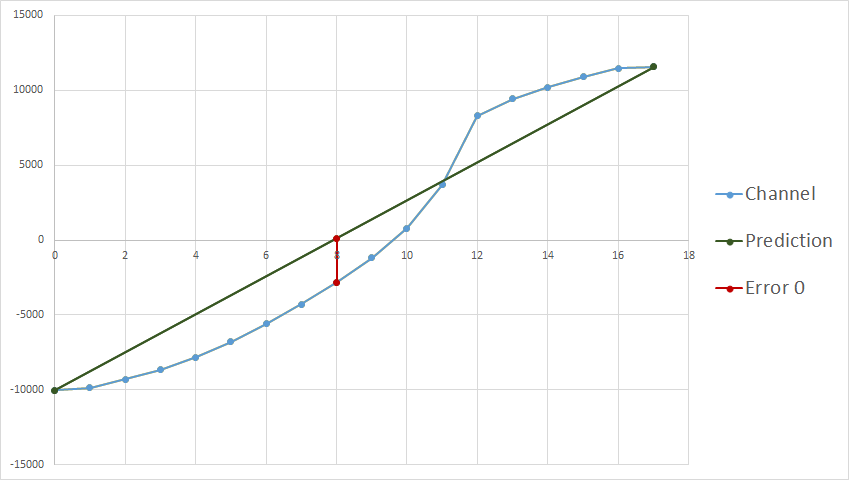
\includegraphics[width=1\textwidth,keepaspectratio]{./pictures/anhang/prediction0.png}
	\caption{First recursive step.}
	\label{anhang:prediction:step1}
\end{figure}
\begin{figure}[!htbp]
	\center
	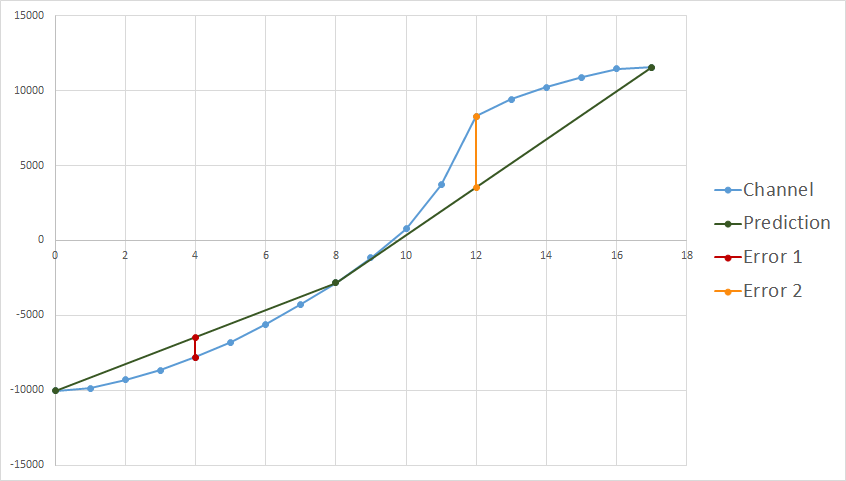
\includegraphics[width=1\textwidth,keepaspectratio]{./pictures/anhang/prediction1.png}
	\caption{Second recursive step.}
	\label{anhang:prediction:step2}
\end{figure}
\begin{table}[!htbp]
	\center
	\begin{tabular}{|c||c|c||c|c|c|c||c}
		\hline
		\multicolumn{8}{|c|}{Prediction Errors of a Channel}\\\hline\hline
		 Step 0& \multicolumn{2}{|c||}{Step 1} & \multicolumn{4}{|c||}{Step 2} &\ldots \\\hline
		$Error_0$ & $Error_1$ &$Fehler_2$ &$Error_3$ & $Error_4$ & $Error_5$ & $Error_6$   & \ldots \\\hline
	\end{tabular}
	\caption{Breadth First ordering.}
	\label{anhang:prediction:breath}
\end{table}
\pagebreak
Here is an example implementation in Java:
\lstinputlisting[language=Java]{./source/prediction.txt}
\pagebreak

\subsection{Performance Tests} \label{anhang:performance}
\begin{table}[!htbp]
\center
\begin{tabular}{c|c}
	Lösunsansatz & Durchschnittliche Dekompressionszeit (ms) \\\hline
	Ist-Zustand & $109$ ms\\
	Adaptives Subsampling & $19$ ms \\
	DCT - Naive Inverse DCT & $3100$ ms \\
	DCT - Mit Kosinus Caching & $65-350$ ms\\
	DCT- Mit JTransform \& Kosinus Caching & $100-135$ ms\\
	Prädiktive Kodierung & $31$ ms\\
\end{tabular}
\end{table}

\textbf{Testmaschine}
\begin{table}[!htbp]
\begin{tabular}{c|c}
	Prozessor & Intel i7-4600 \\
	Arbeitsspeicher & 16 GB \\
	OS & Windows 8.1 Enterprise 64bit \\
\end{tabular}
\end{table}

\textbf{Messverfahren}\\
Die Messung der Dekompression wird mit der Java-Implementation der jeweiligen Verfahren gemessen. Für die Messung wurden die selben Simulationen verwendet wie die der Qualitätsmessung von Abschnitt \ref{testsetup}. Vor der Messung sind die komprimierten Daten bereits im Arbeitsspeicher abgelegt. Vor der Messung wird ein ''Warm-up'' des Hotspot Compilers von Java durchgeführt. Es werden die hälfte der Simulationen dekomprimiert und die Resultate wieder verworfen.